% Intended LaTeX compiler: pdflatex
\documentclass{scrartcl}
    \usepackage{amsmath, amssymb, bm}
		\usepackage[utf8]{inputenc}
		\usepackage[dvipdfmx]{graphicx}
		\usepackage[dvipdfmx]{color}
		\usepackage[backend=biber,bibencoding=utf8]{biblatex}
		\usepackage{url}
		\usepackage{indentfirst}
		\usepackage[normalem]{ulem}
		\usepackage{longtable}
		\usepackage{minted}
		\usepackage{fancyvrb}
    \usepackage[dvipdfmx,colorlinks=true,linkcolor=blue,urlcolor=blue,citecolor=blue,anchorcolor=blue,pdfborder={0 0 0}]{hyperref}
    \usepackage{pxjahyper}
    \usepackage{caption}

		\DeclareMathOperator*{\argmax}{argmax}
\DeclareMathAlphabet{\mathpzc}{OT1}{pzc}{m}{it}
\author{情報科学類3年 江畑 拓哉 (201611350)}
\date{}
\title{オペレーティングシステムⅠ\\\medskip
\large 課題1}
\begin{document}

\maketitle
\section{割り込み処理の必要性とその動作の概要を説明せよ。}
\label{sec:orgef9c163}
 各デバイスとCPUの両者をスムーズに繋ぐために必要で、それ以外にもソフトウェアが発生するエラーやユーザの要求によっても割り込み処理が必要とされている。また、CPUはそれらのデバイスに対して高速に動作するため、CPUの能力を十分に活かすためにもあるデバイスが処理を行っている最中に別のデバイスからの処理を行ったほうが効率が良いことも必要性に挙げられる。\\
 いくつかの割り込み処理は順番に並んでおり、現在ある割り込み処理が呼び出されるとその命令がCPUに渡され実行が行われ、それが終了すると次の割り込み処理に移行していく。また割り込み処理を行う際に、割り込みベクタに次へ飛んでいくアドレスを記述することで自分がすべき命令を見失わないようにしている。\\
\section{記憶装置の階層構造はどういう概念か?図を描いて説明せよ。}
\label{sec:orgb35de0d}
\begin{center}
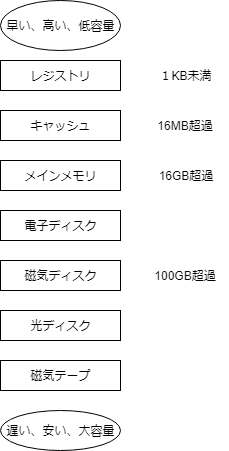
\includegraphics[height=10cm]{./1.png}
\end{center}
上の図のようにレジストリから順に容量が大きく、値段は安く、速度は遅くなっている。\\
尚、効率化のために、下にある物を一時的に上に持ってくることをキャッシングと言う。\\
\section{プログラムライブラリとシステムコールの相違を説明せよ。}
\label{sec:org58cf1f9}
 システムコールはカーネルモード内の動作を行う際に必要なものであり、これはOSに記述されている動作である。対してプログラムライブラリはユーザモードでシステムコールを利用していくためのライブラリであり、これはユーザが作成・変更することが出来る。\\
\end{document}
